%نام و نام خانوادگی:
%شماره دانشجویی: 
\مسئله{مقایسه \lr{LR(1)} و \lr{SLR(1)}}

\پاسخ{

\begin{enumerate}
	\item
	نادرست چون در \lr{slr(1)} کاهش را در مجموعه follow انجام می‌دهد در صورتی که در Lr1 در lookahead که عملا زیر مجموعه فالو است انجام می‌دهد پس تعداد برخورد ها کم می‌شود و با احتمال بیشتری درخت پارس را می‌سازد
	\item
هردو دیاگرام، به شکل زیر خواهند بود و به دلیل رخ دادن \lr{SR Conflict} در حالت 3، نه \lr{SLR(1)} است و نه \lr{LR(1)}.
		\begin{figure}[H]
			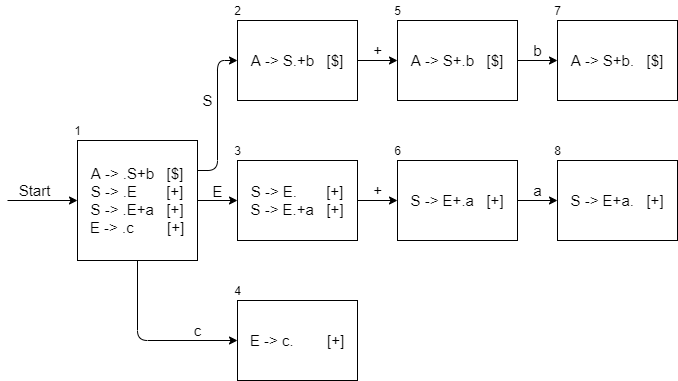
\includegraphics[width=\linewidth]{./commons/Q10.png}
			\label{fig:Q10}
		\end{figure}
\end{enumerate}

}